\documentclass[english,xcolor=svgnames]{beamer}


\input{../Templates/teachingslidesbeamer.tex}



\begin{document}

\title{Sequence Space Methods}
\vspace{1cm}
\author[shortname]{
\begin{tabular}{cc}
Juan Herre\~{n}o & Johannes Wieland \\ 
\end{tabular}\\
}



\date{UCSD, Spring \the\year}

\setbeamertemplate{footline}{}
\makebeamertitle
\setbeamertemplate{footline}[frame number]{}

\addtocounter{framenumber}{-1}



%\begin{frame}
%\frametitle[alignment=center]{Reminders}
%\begin{enumerate}
%	\item First project draft due May 1.
%	\item Participation.
%\end{enumerate}
%\end{frame}


%%%%%%%%%%%%%%%%%%%%%%%%%%%%%%%%%%%%%%%%%%%%%%%%%%
\AtBeginSection[]{
\setbeamertemplate{footline}{}
  \frame<beamer>{ 

    \frametitle{Outline}   

    \tableofcontents[currentsection,hideallsubsections] 
  }
\setbeamertemplate{footline}[frame number]{}
\addtocounter{framenumber}{-1}
}

\AtBeginSubsection[]{
\setbeamertemplate{footline}{}
  \frame<beamer>{ 

    \frametitle{Outline}   

    \tableofcontents[currentsection,currentsubsection] 
  }
  \setbeamertemplate{footline}[frame number]{}
  \addtocounter{framenumber}{-1}
}



\setbeamertemplate{footline}{}
\begin{frame}
\frametitle{Outline}   
\tableofcontents[hideallsubsections] 
\end{frame}
\addtocounter{framenumber}{-1}
\setbeamertemplate{footline}[frame number]{}


%%%%%%%%%%%%%%%%%%%%%%%%%%%%%%%%%%%%%%%%%%%%%%%%%%
\section{Introduction}
%%%%%%%%%%%%%%%%%%%%%%%%%%%%%%%%%%%%%%%%%%%%%%%%%%

\begin{frame}
   \frametitle{Introduction}
   \begin{itemize}
       \item We will learn how to solve models in sequence space.
       \item Basic idea: organize models into ``blocks'' that represent behavior of (possibly heterogeneous) agents, and interact in GE via a small set of aggregates.
       \item We will arrange these blocks into Directed Acyclic Graph (``DAG''). Helpful to solve model, think about causality in GE, do decompositions, etc.
       \item Very useful for solving HA models (not today).
   \end{itemize}
   \centering
   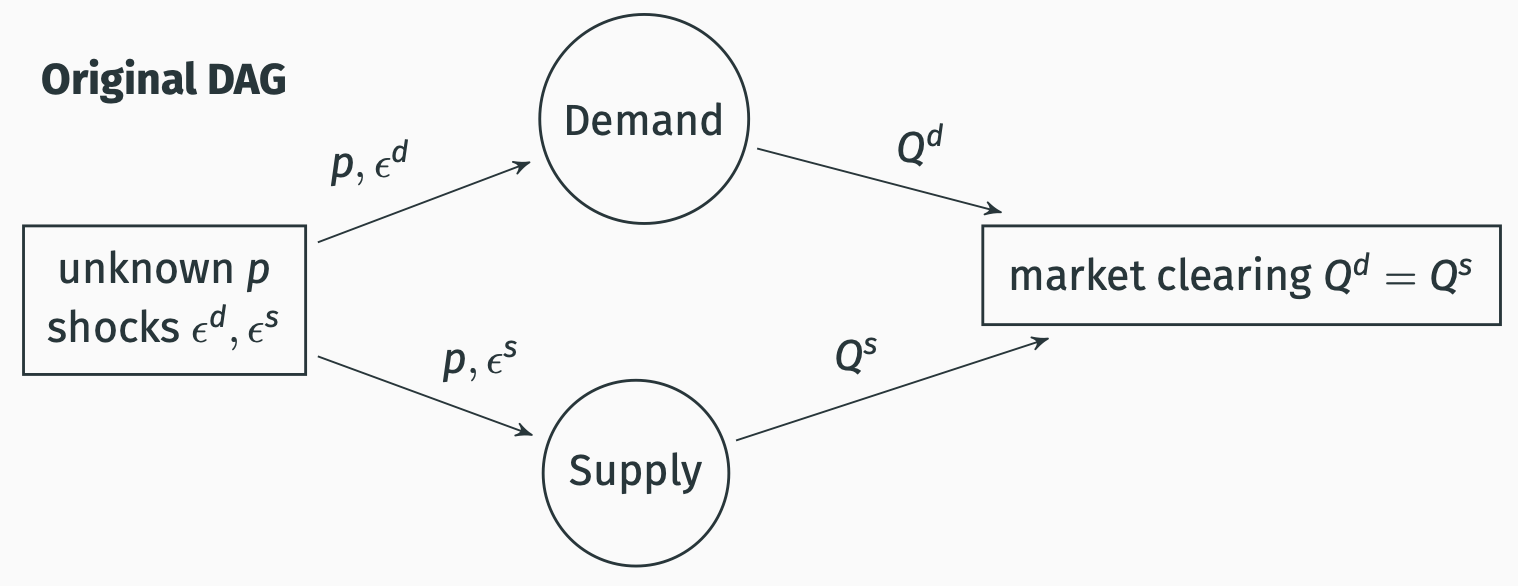
\includegraphics[scale=0.3]{dag/demandsupply.png}
\end{frame}

%%%%%%%%%%%%%%%%%%%%%%%%%%%%%%%%%%%%%%%%%%%%%%%%%%
\section{State Space}
%%%%%%%%%%%%%%%%%%%%%%%%%%%%%%%%%%%%%%%%%%%%%%%%%%

\begin{frame}
   \frametitle{State Space Approach}
   \begin{itemize}
	   \item You are likely more familiar with the state space approach.
       \item Solve for policies and prices as functions of the state.
       \item State: what is given to you today.
       \item Policy: what you chose based on FOC.
       \item Prices: those that implement the equilibrium (market clearing)
       \item Requires specifying a law of motion for the exogenous states.
	\end{itemize}
\end{frame}

\begin{frame}
	\frametitle{General State Space Representation}
	\begin{itemize}
		\item State space representation of a linearized macro model (including HANK) is:
		\begin{align*}
			A \begin{pmatrix} x_{t+1} \\
				E_t y_{t+1}
		\end{pmatrix}
			+ B \begin{pmatrix} x_{t} \\
				y_{t}
		\end{pmatrix} &= \begin{pmatrix} \epsilon_{t+1} \\
			0
	\end{pmatrix}  
		\end{align*}
		\begin{itemize}
			\item $x_t$ is an $n-m\times 1$ vector of predetermined variables.
			\item $y_t$ is an $m\times 1$ vector of jump/policy variables.
		\end{itemize}
	 \end{itemize}
 \end{frame}

 \begin{frame}
	\frametitle{Neoclassical Growth Model}
	\begin{itemize}
		\item Euler equation:
		\begin{align*}
			C_t^{-\gamma}  = \beta E_t C_{t+1}^{-\gamma} (1-\delta+MPK_{t+1}^k)
		\end{align*}
		\item Law of motion for capital:
		\begin{align*}
			K_{t} = I_t + (1-\delta)K_{t-1}
		\end{align*}
		\item Production function:
		\begin{align*}
			Y_t = Z_t K_{t-1}^\alpha
		\end{align*}
		\item Return to capital:
		\begin{align*}
			MPK_{t+1}^k = \alpha Z_{t+1} K_t^{\alpha-1}
		\end{align*}
		\item Market clearing:
		\begin{align*}
			Y_t = C_t + I_t
		\end{align*}
	 \end{itemize}
 \end{frame}

 \begin{frame}
	\frametitle{Neoclassical Growth Model Linearized}
	\begin{itemize}
		\item Euler equation:
		\begin{align*}
			-\gamma \hat{c}_t &= -\gamma \E_t \hat{c}_{t+1} + (1 - \beta(1-\delta)) \E_t \hat{mpk}_{t+1}
		\end{align*}
		\item Law of motion for capital:
		\begin{align*}
			\hat{k}_{t} =\delta \hat{\iota}_{t} + (1-\delta)\hat{k}_{t-1}
		\end{align*}
		\item Production function:
		\begin{align*}
			\hat{y}_t = \hat{z}_t + \alpha \hat{k}_{t-1}
		\end{align*}
		\item Return to capital:
		\begin{align*}
			\hat{mpk}_{t+1} =  \hat{z}_{t+1} + (\alpha-1) \hat{k}_t 
		\end{align*}
		\item Market clearing:
		\begin{align*}
			\hat{y}_t = s_c \hat{c}_t +(1-s_c) \hat{\iota}_t
		\end{align*}
	 \end{itemize}
 \end{frame}

\begin{frame}
	\frametitle{Solving State Space}
	\begin{itemize}
		\item How to solve this?
		\begin{align*}
			\begin{pmatrix} x_{t+1} \\
				E_t y_{t+1}
		\end{pmatrix} &= 
			-A^{-1}B \begin{pmatrix} x_{t} \\
				y_{t}
		\end{pmatrix} + A^{-1} \begin{pmatrix} \epsilon_{t+1} \\
			0
	\end{pmatrix}  \\
	&=VD^{-1}V^{-1} \begin{pmatrix} x_{t} \\
		y_{t}
\end{pmatrix} + A^{-1} \begin{pmatrix} \epsilon_{t+1} \\
	0
\end{pmatrix}  \\
	\begin{pmatrix} \tilde{x}_{t+1} \\
		E_t \tilde{y}_{t+1}
\end{pmatrix} &= 
	D \begin{pmatrix} \tilde{x}_{t} \\
		\tilde{y}_{t}
\end{pmatrix} + V^{-1}A^{-1} \begin{pmatrix} \epsilon_{t+1} \\
	0
\end{pmatrix}  
		\end{align*}
		\item Solve $\tilde{x}$ backward and $\tilde{y}$ forward. Then rotate back using
		\begin{align*}
			\begin{pmatrix} x_{t+1} \\
				E_t y_{t+1}
		\end{pmatrix} \equiv V^{-1} \begin{pmatrix} \tilde{x}_{t+1} \\
			E_t \tilde{y}_{t+1}
	\end{pmatrix} 
		\end{align*}
		\item Unique stable solution if number of eigenvalues $D$ inside unit circle is $n-m$.
		\item Dimension of the problem is $n\times n$.
	 \end{itemize}
 \end{frame}




%%%%%%%%%%%%%%%%%%%%%%%%%%%%%%%%%%%%%%%%%%%%%%%%%%
\section{Sequence Space}
%%%%%%%%%%%%%%%%%%%%%%%%%%%%%%%%%%%%%%%%%%%%%%%%%%

\begin{frame}
    \frametitle{General Sequence Space Representation}
    \begin{itemize}
        \item Equilibrium is a solution to an equation
        \begin{align*}
        	\mathbf{H}(\mathbf{U}, \mathbf{Z}) = 0
        \end{align*}
        where
        \begin{itemize}
        	\item $\mathbf{U}$ represents the time path $U_0,U_1,...,$ of unknown aggregate sequences (e.g., quantities, prices).
        	\item $\mathbf{Z}$ represents the time path $Z_0,Z_1,...,$ of known exogenous shocks.
        \end{itemize}
        \item Totally differentiate and evaluate at steady state to get:
        \begin{align*}
        	d\mathbf{U} = -\mathbf{H}_{\mathbf{U}}(\mathbf{\bar{U}}, \mathbf{\bar{Z}})^{-1}\mathbf{H}_{\mathbf{Z}}(\mathbf{\bar{U}}, \mathbf{\bar{Z}})d\mathbf{Z}
        \end{align*}
        \item Solution requires finding the sequence-space Jacobians $\mathbf{H}_{\mathbf{U}}$ and $\mathbf{H}_{\mathbf{Z}}$.
	\end{itemize}
\end{frame}



\begin{frame}
    \frametitle{Sequence Space Approach}
    \begin{itemize}
        \item Solve for sequences of policies and prices given a known sequence of exogenous shocks.
        \item Aligns closely with equilibrium definition.
        \item Dimension of the problem is $T \times \text{number of variables}$.
       \item Unlike state space we do not solve for a function of the state.
       \begin{itemize}
		\item This can be helpful when the state is very high-dimensional
	   \end{itemize}
        % \item Typically used in heterogeneous agent literature where characterizing the equilibrium as a function of the state is difficult. 
        \item The sequence space approach assumes perfect foresight. 
        \begin{itemize}
			\item Can get around this to some extent using ``MIT-shocks.''
		   \end{itemize}
	\end{itemize}
\end{frame}

\begin{frame}
	\frametitle{Neoclassical Growth Model Linearized}
	\begin{itemize}
		\item Repeated substitution:
		\begin{align*}
			0=H_t(\mathbf{\hat{K}},\mathbf{\hat{Z}})&\equiv  \gamma\left[\alpha + (1-s_c)\frac{1-\delta}{\delta}\right]\hat{k}_{t-1} \\
			&-\gamma \left[\alpha + (1-s_c)\frac{1}{\delta}+(1-\alpha)s_c(1 - \beta(1-\delta))\right]\hat{k}_{t} \\
			&   +\gamma  (1-s_c)\frac{1}{\delta}\hat{k}_{t+1} \\
			&+ \gamma \hat{z}_t \\
			& -\left[\gamma-s_c(1 - \beta(1-\delta)) \right]  \hat{z}_{t+1} 
		\end{align*}
	 \item The H-matrix is:
		\begin{align*}
			\mathbf{0} = \mathbf{H}(\mathbf{\hat{K}},\mathbf{\hat{Z}}) \equiv \begin{pmatrix}
				H_0(\mathbf{\hat{K}},\mathbf{\hat{Z}}) \\
				H_1(\mathbf{\hat{K}},\mathbf{\hat{Z}}) \\
				\vdots \\
				H_T(\mathbf{\hat{K}},\mathbf{\hat{Z}})
			\end{pmatrix}
		\end{align*}
		\end{itemize}
 \end{frame}

% \begin{frame}
% 	\frametitle{Neoclassical Growth Model in Sequence Space}
% 	\begin{itemize}
		
		
% 	 \end{itemize}
%  \end{frame}



\begin{frame}
	\frametitle{Exercise 1: Neoclassical Growth Model}
	\begin{enumerate}
		\item Derive $\mathbf{H}_\mathbf{\hat{K}} = \begin{pmatrix}
			\frac{\partial H_0(\mathbf{\hat{K}})}{\partial \hat{k}_0} & \frac{\partial H_0(\mathbf{\hat{K}})}{\partial \hat{k}_1} & \hdots & \frac{\partial H_0(\mathbf{\hat{K}})}{\partial \hat{k}_T} \\
			\frac{\partial H_1(\mathbf{\hat{K}})}{\partial \hat{k}_0} & \frac{\partial H_1(\mathbf{\hat{K}})}{\partial \hat{k}_1} & \hdots & \frac{\partial H_1(\mathbf{\hat{K}})}{\partial \hat{k}_T} \\
			\vdots & \vdots & \ddots & \vdots \\
			\frac{\partial H_T(\mathbf{\hat{K}})}{\partial \hat{k}_0} & \frac{\partial H_T(\mathbf{\hat{K}})}{\partial \hat{k}_1} & \hdots & \frac{\partial H_T(\mathbf{\hat{K}})}{\partial \hat{k}_T} \\
		\end{pmatrix}$
		\item Derive $\mathbf{H}_\mathbf{\hat{Z}} = \begin{pmatrix}
			\frac{\partial H_0(\mathbf{\hat{K}})}{\partial \hat{z}_0} & \frac{\partial H_0(\mathbf{\hat{K}})}{\partial \hat{z}_1} & \hdots & \frac{\partial H_0(\mathbf{\hat{K}})}{\partial \hat{z}_T} \\
			\frac{\partial H_1(\mathbf{\hat{K}})}{\partial \hat{z}_0} & \frac{\partial H_1(\mathbf{\hat{K}})}{\partial \hat{z}_1} & \hdots & \frac{\partial H_1(\mathbf{\hat{K}})}{\partial \hat{z}_T} \\
			\vdots & \vdots & \ddots & \vdots \\
			\frac{\partial H_T(\mathbf{\hat{K}})}{\partial \hat{z}_0} & \frac{\partial H_T(\mathbf{\hat{K}})}{\partial \hat{z}_1} & \hdots & \frac{\partial H_T(\mathbf{\hat{K}})}{\partial \hat{z}_T} \\
		\end{pmatrix}$
		\item Assume $\hat{z}_t$ is an AR(1) with persistence $\rho_z = 0.9$. Compute and plot $\mathbf{\hat{k}}$.
	 \end{enumerate}
 \end{frame}


% \begin{frame}
%     \frametitle{Sequence Space Representation of RBC}
%     \begin{itemize}
%         \item At every point in time:
%         \begin{align*}
% 	\mathbf{H}_t(\mathbf{\hat{c}},\mathbf{\hat{a}}) &= \begin{pmatrix} (\gamma+\varphi)\hat{c}_t - (1+\varphi)\hat{a}_t  \\
% 	 \hat{r}_{t+1} -  \gamma (\hat{c}_{t+1} - \hat{c}_{t}) \end{pmatrix} = \begin{pmatrix}
% 		0 \\ 0
% 	\end{pmatrix} ,\qquad \forall t\ge 0
% \end{align*}
% 	\item First write every equation individually in sequence space:
% 	\hspace{-2cm}\begin{align*}
% 		 (\gamma + \phi)\begin{pmatrix}
% 	1 & 0 & \hdots & 0 \\
% 	0 & 1 & \ddots & 0 \\
% 	\vdots & 0 & \ddots & 0 \\
% 	0 & 0 & \hdots & 1 \\	
% \end{pmatrix}\begin{pmatrix}
% 	\hat{c}_0 \\
% 	\hat{c}_1 \\
% 	\vdots \\
% 	\hat{c}_T \\	
% \end{pmatrix} - (1 + \phi)\begin{pmatrix}
% 	1 & 0 & \hdots & 0 \\
% 	0 & 1 & \ddots & 0 \\
% 	\vdots & 0 & \ddots & 0 \\
% 	0 & 0 & \hdots & 1 \\	
% \end{pmatrix}\begin{pmatrix}
% 	\hat{a}_0 \\
% 	\hat{a}_1 \\
% 	\vdots \\
% 	\hat{a}_T \\	
% \end{pmatrix} = \begin{pmatrix}
% 	0 \\
% 	0 \\
% 	0 \\
% 	0 \\	
% \end{pmatrix}\\
% \gamma\begin{pmatrix}
% 	1 & -1 & 0 & \hdots & 0 \\
% 	0 & 1 & -1 & \ddots & 0 \\
% 	\vdots &  0 & \ddots & \ddots & 0 \\
% 	0 & 0 & \ddots & 1 & -1 \\	
% 	0 & 0 & \hdots & 0 & 1 \\	
% \end{pmatrix}\begin{pmatrix}
% 	\hat{c}_0 \\
% 	\hat{c}_1 \\
% 	\vdots \\
% 	\hat{c}_T \\	
% \end{pmatrix} + \begin{pmatrix}
% 	1 & 0 & 0 & \hdots & 0 \\
% 	0 & 1 & 0 &\ddots & 0 \\
% 	\vdots & 0 & \ddots & \ddots & 0 \\
% 	0 & 0 & \ddots & 1 & 0 \\	
% 	0 & 0 & \hdots & 0 & 1 \\	
% \end{pmatrix}\begin{pmatrix}
% 	\hat{r}_0 \\
% 	\hat{r}_1 \\
% 	\vdots \\
% 	\hat{r}_T \\	
% \end{pmatrix} = \begin{pmatrix}
% 	0 \\
% 	0 \\
% 	0 \\
% 	0 \\	
% \end{pmatrix}
% 	\end{align*}
% 	\end{itemize}
% \end{frame}

% %%%%%%%%%%%%%%%%%%%%%%%%%%%%%%%%%%%%%%%%%%%%%%%%%%
% \section{Solving RBC in Sequence Space}
% %%%%%%%%%%%%%%%%%%%%%%%%%%%%%%%%%%%%%%%%%%%%%%%%%%

% \begin{frame}
%     \frametitle{Solving RBC in Sequence Space}
%     \begin{itemize}
%         \item Simplify as
%         \begin{align*}
% 		 \mathbf{A}\mathbf{\hat{c}} + \mathbf{B} \mathbf{\hat{a}} = \mathbf{0}\\
% \mathbf{C}\mathbf{\hat{c}} + \mathbf{D}\mathbf{\hat{r}} = \mathbf{0}
% 	\end{align*}
% 	\item One approach is to stack everything.
% 	\begin{align*}
% 		\begin{pmatrix}
% 			\mathbf{A} & \mathbf{0} \\
% 			\mathbf{C} & \mathbf{D}
% 		\end{pmatrix}\begin{pmatrix}
% 			\mathbf{\hat{c}} \\
% 			\mathbf{\hat{r}}
% 		\end{pmatrix} + \begin{pmatrix}
% 			\mathbf{B} \\ \mathbf{0} 
% 		\end{pmatrix}\begin{pmatrix}
% 			\mathbf{\hat{a}}
% 		\end{pmatrix} = \mathbf{0}
% 	\end{align*}
%       \item This is linear algebra.
%       \begin{align*}
%       	\begin{pmatrix}
% 			\mathbf{\hat{c}} \\
% 			\mathbf{\hat{r}}
% 		\end{pmatrix} = \begin{pmatrix}
% 			\mathbf{A} & \mathbf{0} \\
% 			\mathbf{C} & \mathbf{D}
% 		\end{pmatrix}^{-1} \begin{pmatrix}
% 			-\mathbf{B} \\ \mathbf{0} 
% 		\end{pmatrix}\begin{pmatrix}
% 			\mathbf{\hat{a}}
% 		\end{pmatrix} = \begin{pmatrix}
% 			-\mathbf{A}^{-1}\mathbf{B} \\ \mathbf{D}^{-1} \mathbf{C}\mathbf{A}^{-1}\mathbf{B}
% 		\end{pmatrix}\begin{pmatrix}
% 			\mathbf{\hat{a}}
% 		\end{pmatrix}
%       \end{align*}
%       \end{itemize}
% \end{frame}

%\begin{frame}
%    \frametitle{Sequence Space Approach}
%    \begin{itemize}
%        \item Why don't we just do $\mathbf{\hat{c}}=\mathbf{A}^{-1}\mathbf{B}\mathbf{\hat{a}}$ and then substitute?
%        \item Indeed we should! 
%        \item The computer can do this for us as well, which is helpful for more complex models.
%        \item We will see this idea is closely connected to the Directed Acyclical Graph (DAG) representation, which is useful way to organize models.
%	\end{itemize}
%\end{frame}




%\begin{frame}
%    \frametitle{Objective}
%    \begin{itemize}
%        \item Hard when there is rich heterogeneity.
%        \item Infinitely dimensional state space from the distribution of agent's endogenous state variables---how to handle it?
%        \item In macro, we are often interested what happens when aggregate shock X hits the economy (monetary, fiscal, etc).
%        \item State space: must forecast infinite-dimensional distribution to estimate prices / quantities relevant to agents' problem.
%        \item Sequence space: must find price / quantity sequences that solve market clearing conditions.
%        \item[$\Rightarrow$] Sequence space is of dimension $T \times \text{number of variables}$, versus infinite dimensional state space. 
%       	\item Cost: linearization / perfect foresight.
%    \end{itemize}
%\end{frame}



%%%%%%%%%%%%%%%%%%%%%%%%%%%%%%%%%%%%%%%%%%%%%%%%%%
\section{DAG Representation}
%%%%%%%%%%%%%%%%%%%%%%%%%%%%%%%%%%%%%%%%%%%%%%%%%%

\begin{frame}
	\frametitle{Solving in Sequence Space}
	\begin{itemize}
		\item Organize the model in blocks.
		\begin{enumerate}
			\item Firm block:
			\begin{align*}
				\hat{y}_t &= \hat{z}_t + \alpha \hat{k}_{t-1} \\
				\hat{mpk}_{t+1} &=  \hat{z}_{t+1} + (\alpha-1) \hat{k}_t 
			\end{align*}
			\item Household block:
			\begin{align*}
				\hat{k}_{t} &=\delta \hat{\iota}_{t-1} + (1-\delta)\hat{k}_t \\
				- \gamma \hat{c}_t &= -\gamma  \hat{c}_{t+1} + (1 - \beta(1-\delta))  \hat{mpk}_{t+1} 
			\end{align*}
			\item Market clearing block:
			\begin{align*}
				0&=s_c \hat{c}_t +(1-s_c) \hat{\iota}_t - \hat{y}_t 
			\end{align*}
		\end{enumerate}
	\end{itemize}
	\end{frame}


	
	\begin{frame}
		\frametitle{Sequence Space Algorithm Heuristics}
			\begin{enumerate}
				\item Start with an initial guess of the sequences $(\mathbf{\hat{k}})=\{\hat{k}_{t}\}_{t=0}^{\infty}$.
				\begin{itemize}
					\item $\mathbf{\hat{a}}=\{a_t\}_{t=0}^{\infty}$ and $\hat{k}_{t-1}$ are given to us.
				\end{itemize}
				\item Solve the firm block for $\mathbf{\hat{y}}$ and $\mathbf{\hat{mpk}}$.
				\item Solve the household block for $\mathbf{\hat{c}}$, $\mathbf{\hat{\iota}}$.
				\item Check that market clears. If not update guess $\mathbf{\hat{k}}$
				\begin{itemize}
					\item In turns out we do not need to guess, but can solve the entire system with linear algebra in one step.
					\item Approach follows equilibrium definition: find sequences such that everyone optimizes and markets clear.
				\end{itemize}
			\end{enumerate}
	\end{frame}
	
	\begin{frame}
		\frametitle{DAG Representation}
			\begin{itemize}
				\item Effectively what we have done is organized our model in a Directed Acyclical Graph (DAG).
			\end{itemize}
			\centering
			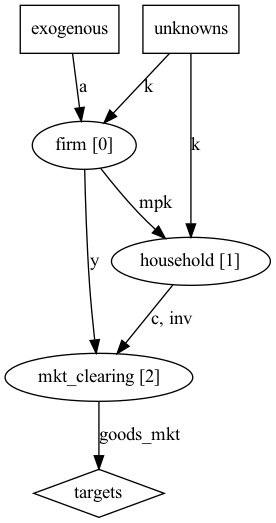
\includegraphics[scale=0.4]{dag/neoclassical.png}
	\end{frame}

	\begin{frame}
		\frametitle{DAG Rules}
			\begin{itemize}
				\item There are no cycles in a DAG---we travel in one direction only.
				\item A model has many DAG representations.
				\begin{itemize}
					\item One representation is to treat every endogenous variable as unknown and have single block.
					\item Another representation is to treat each equation as an individual block.
					\item These are often not the most useful representation.
				\end{itemize}
			\end{itemize}
	\end{frame}
	
	\begin{frame}
		\frametitle{DAG Suggestions}
			\begin{itemize}
				\item A good DAG minimizes the number of unknowns.
				\item Generally useful to organize blocks by agent: household, firm, union, government, market clearing.
				\item Blocks make updating the model easy. Often we change just one problem (e.g., firm for NK model) and leave others untouched.
				\item Logical check for each block: are the number of variables to solve for equal to the number of equations?
				\item The computer can organize our model in a DAG and substitute for us.
				\item Today we will see what the computer does under the hood.
			\end{itemize}
	\end{frame}

%%%%%%%%%%%%%%%%%%%%%%%%%%%%%%%%%%%%%%%%%%%%%%%%%%
\section{Moving Along the DAG}
%%%%%%%%%%%%%%%%%%%%%%%%%%%%%%%%%%%%%%%%%%%%%%%%%%

	\begin{frame}
		\frametitle{Solving in Sequence Space}
			\begin{itemize}
				\item We want to clear markets at all points in time:
				\begin{align*}
					\mathbf{H} = \begin{pmatrix}
						s_c \hat{c}_0 +(1-s_c) \hat{\iota}_0- \hat{y}_0 \\
						\vdots \\
						s_c \hat{c}_T +(1-s_c) \hat{\iota}_T  - \hat{y}_T \\
					\end{pmatrix} = \begin{pmatrix}
						\Phi_{gm,c}\mathbf{\hat{c}} + \Phi_{gm,c}\mathbf{\hat{\iota}} +  \Phi_{gm,y}\mathbf{\hat{y}} 
					\end{pmatrix} = \mathbf{0}
				\end{align*}
				where
				\begin{align*}
					\Phi_{gm,c} &= s_c I_T \\
					\Phi_{gm,\iota} &= (1 - s_c) I_T \\
					\Phi_{gm,y} &= -I_T
				\end{align*}
				and $I_T$ is the $T\times T$ identity matrix.
				\item How does adjusting the sequences $\mathbf{U} = (\mathbf{\hat{k}})$ change the target?
				\begin{align*}
					\mathbf{H}_{\mathbf{U}} = \begin{pmatrix}
						\Phi_{gm,c}\frac{\partial\mathbf{\hat{c}}}{\partial \mathbf{\hat{k}} } + \Phi_{gm,\iota}\frac{\partial\mathbf{\hat{\iota}}}{\partial \mathbf{\hat{k}} } +  \Phi_{gm,y}\frac{\partial\mathbf{\hat{y}}}{\partial \mathbf{\hat{k}} }
					\end{pmatrix}
				\end{align*}
	%			\item These are all objects we can compute.
			\end{itemize}
	\end{frame}
	
	
	\begin{frame}
		\frametitle{Solving in Sequence Space}
			\begin{itemize}
				\item A simpler and equivalent expression to work with is
				\begin{align*}
					\mathbf{H}_{\mathbf{U}} = \begin{pmatrix}
						\Phi_{gm,c} & \Phi_{gm,\iota} & \Phi_{gm,y}  & \mathbf{0}_T 
					\end{pmatrix}
					\begin{pmatrix}
						\frac{\partial\mathbf{\hat{c}}}{\partial \mathbf{\hat{k}} } \\ 
						\frac{\partial\mathbf{\hat{\iota}}}{\partial \mathbf{\hat{k}} } \\ 
						\frac{\partial\mathbf{\hat{y}}}{\partial \mathbf{\hat{k}} } \\
						\frac{\partial\mathbf{\hat{mpk}}}{\partial \mathbf{\hat{k}} } 
					\end{pmatrix} \equiv \frac{\partial \mathbf{H}}{\partial \mathbf{Y}}\frac{\partial \mathbf{Y}}{\partial \mathbf{U}}
				\end{align*}
				\item Now we move along using the chain rule:
				\begin{align*}
					\frac{\partial \mathbf{Y}}{\partial \mathbf{U}} = \begin{pmatrix}
						\frac{\partial \mathbf{(c,\iota)}}{\partial \mathbf{U}} \\
						\frac{\partial (\mathbf{\hat{y}},\mathbf{(\hat{w}-\hat{p})})}{\partial \mathbf{U}}\\
					\end{pmatrix} \\
				\end{align*}
				where we partitioned based on the two blocks we looked at earlier.
			\end{itemize}
	\end{frame}
	
	\begin{frame}
    \frametitle{Solving in Sequence Space}
		\begin{itemize}
			\item We start with the firm block:
			\begin{align*}
				\hat{y}_t&=\hat{a}_t +\alpha \hat{k}_{t-1} 
			\end{align*}
			\item In matrix notation:
			\begin{align*}
				\mathbf{\hat{y}} &= \mathbf{\hat{z}} + \Phi_{y,k}\mathbf{\hat{k}} + \Phi_{y,k_{-1}}\hat{k}_{-1}
			\end{align*}
			\item The matrices are:
			\begin{align*}
				\Phi_{y,k}&=\alpha \begin{pmatrix} 
					0 & 0 & \hdots & 0 & 0 \\
					1 & 0 & \hdots & 0 & 0 \\
					0 & 1 & \ddots & 0 & 0 \\
					\vdots & \ddots & \ddots & 0 & 0 \\
					0 & 0 & \hdots & 1 & 0
				\end{pmatrix},\; 
				\Phi_{y,k_{-1}}=\begin{pmatrix}
					1 & 0 & \hdots & 0 \\
					0 & 0 & \hdots & 0 \\
					\vdots & \vdots & \ddots & 0 \\
					0 & 0 & \hdots & 0
				\end{pmatrix}
			\end{align*}
			\item Note timing!
		\end{itemize}
\end{frame}
	
	\begin{frame}
		\frametitle{Solving in Sequence Space}
			\begin{itemize}
				\item The second equation in the firm block:
				\begin{align*}
					\hat{mpk}_{t+1} &=  \hat{z}_{t+1} + (\alpha-1) \hat{k}_t 
				\end{align*}
				\item In matrix notation:
				\begin{align*}
					\mathbf{\hat{mpk}} &= \Phi_{mpk,z}\mathbf{\hat{z}} + \Phi_{mpk,z}\mathbf{\hat{k}}
				\end{align*}
				\item The matrices are:
				\begin{align*}
					\Phi_{mpk,z}&=\begin{pmatrix}
						0 & 1 & 0 & \hdots & 0  \\
						0 & 0 & 1 & \hdots & 0  \\
						\vdots & \vdots & \ddots & \ddots & \vdots  \\
						0 & 0 & 0 & \ddots & 1  \\
						0 & 0 & 0 & \hdots & 0 
					\end{pmatrix} \\
					\Phi_{mpk,z}&=(\alpha-1)  I_T 
				\end{align*}
				\item Note timing!
			\end{itemize}
	\end{frame}

	
	\begin{frame}
		\frametitle{Solving in Sequence Space}
			\begin{itemize}
				\item With $\mathbf{\hat{mpk}}$ and $\mathbf{\hat{k}}$  we solve for $\mathbf{\hat{c}}$ and $\mathbf{\hat{\iota}}$ using the household FOC.
				\item Start with investment:
				\begin{align*}
					\hat{k}_{t} &=\delta \hat{\iota}_t + (1-\delta)\hat{k}_{t-1} \\
				\end{align*}
				\item In matrix notation:
				\begin{align*}
					\mathbf{\hat{\iota}} &= \Phi_{\iota,k}\mathbf{\hat{k}} + \Phi_{\iota,k{-1}}\hat{k}_{-1} \\
				\end{align*}
				\item The matrix is:
				\begin{align*}
					\Phi_{\iota,k}&=\delta^{-1}\begin{pmatrix} 1 & 0 & \hdots & 0 & 0 \\
						\delta-1 & 1 & \hdots & 0 & 0 \\
						0 & \delta-1 & \ddots & 0 & 0 \\
						\vdots & \ddots & \ddots & 1 & 0 \\
						0 & 0 & \hdots & \delta-1 & 1
					\end{pmatrix}
				\end{align*}
			\end{itemize}
	\end{frame}

	\begin{frame}
		\frametitle{Solving in Sequence Space}
			\begin{itemize}
				\item Next consumption:
				\begin{align*}
					- \gamma \hat{c}_t &= -\gamma  \hat{c}_{t+1} + (1 - \beta(1-\delta))  \hat{mpk}_{t+1} 
				\end{align*}
				\item In matrix notation:
				\begin{align*}
					\mathbf{\hat{c}} &= \Phi_{c,mpk}\mathbf{\hat{mpk}} 
				\end{align*}
				\item The matrices are:
				\begin{align*}
					\Phi_{c,mpk}&=-\gamma^{-1}(1-\beta(1-\delta))\begin{pmatrix}
						1 & -1 & 0 & \hdots & 0  \\
						0 & 1 & -1 & \hdots & 0  \\
						\vdots & \vdots & \ddots & \ddots & \vdots  \\
						0 & 0 & \hdots & 1 & -1 \\
						0 & 0 & \hdots & 0 & 1 \\
					\end{pmatrix}^{-1}
				\end{align*}
			\end{itemize}
	\end{frame}
	
	
	
	
	\begin{frame}
		\frametitle{Solving in Sequence Space}
			\begin{itemize}
				\item From the firm block we have:
				\begin{align*}
					\frac{\partial (\mathbf{\hat{y}},\mathbf{(\hat{mpk})})}{\partial \mathbf{U}} = \begin{pmatrix}
						\Phi_{y,k} \\
						\Phi_{mpk,k} \\
					\end{pmatrix}
				\end{align*}
				\item From the household block we have:
				\begin{align*}
					\frac{\partial \mathbf{(\hat{c},\hat{\iota})}}{\partial \mathbf{U}} &= \begin{pmatrix}
						\Phi_{c,mpk}\frac{d\mathbf{\hat{mpk}}}{\partial \mathbf{\hat{k}} } \\
						\Phi_{\iota,k} \\
					\end{pmatrix} \\
					&= \begin{pmatrix}
						\Phi_{c,mpk}\Phi_{mpk,k} \\
						\Phi_{\iota,k} \\
					\end{pmatrix}
				\end{align*}
				\item We solved for $\mathbf{H}_{\mathbf{U}}$:
				\begin{align*}
					\mathbf{H}_{\mathbf{U}} =&\begin{pmatrix}
						\Phi_{gm,c} & \Phi_{gm,\iota} & \Phi_{gm,y}  & \mathbf{0}_T   \\ 
					\end{pmatrix} \times  \begin{pmatrix}
						\Phi_{c,mpk}\Phi_{mpk,k} \\
						\Phi_{\iota,k} \\
						\Phi_{y,k} \\
						\Phi_{mpk,k} \\
					\end{pmatrix} \\
					= &\begin{pmatrix}
						\Phi_{gm,c}\Phi_{c,mpk}\Phi_{mpk,k} + \Phi_{gm,\iota}\Phi_{\iota,k} - \Phi_{y,k} 
					\end{pmatrix} 
				\end{align*}
			\end{itemize}
	\end{frame}
	
	
	
	\begin{frame}
		\frametitle{Solving in Sequence Space}
			\begin{itemize}
				\item Solving for $\mathbf{H}_{\mathbf{Z}}$ is a bit more straightforward:
				\begin{align*}
					\mathbf{H}_{\mathbf{Z}} = \frac{\partial \mathbf{H}}{\partial \mathbf{Y}}\frac{\partial \mathbf{Y}}{\partial \mathbf{Z}} \\
				\end{align*}
				We already know the first derivative.
				\item From the firm block we have:
				\begin{align*}
					\frac{\partial \mathbf{\hat{y}}}{\partial \mathbf{Z}} = I_T
				\end{align*}
				and
				\begin{align*}
					\frac{\partial \mathbf{(\hat{mpk})}}{\partial \mathbf{Z}}=\Phi_{mpk,z} = \begin{pmatrix}
						 0 & 1 & 0 & \hdots & 0  \\
						0 & 0 & 1 & \hdots & 0  \\
						\vdots & \vdots & \ddots & \ddots & \vdots  \\
						0 & 0 & 0 & \ddots & 1  \\
						0 & 0 & 0 & \hdots & 0
					\end{pmatrix}
				\end{align*}
			\end{itemize}
	\end{frame}
	

	\begin{frame}
		\frametitle{Solving in Sequence Space}
			\begin{itemize}
				\item From the household block we have:
				\begin{align*}
					\frac{\partial \mathbf{\hat{c},\hat{\iota}}}{\partial \mathbf{Z}} &= \begin{pmatrix}
						\Phi_{c,wp}\frac{\partial\mathbf{\hat{mpk}}}{\partial \mathbf{\hat{z}} } \\
						\mathbf{0}_T \\
					\end{pmatrix} = \begin{pmatrix}
						\Phi_{c,mpk}\Phi_{mpk,z} \\
						\mathbf{0}_T \\
					\end{pmatrix}
				\end{align*}
				\item We solved for $\mathbf{H}_{\mathbf{Z}}$:
				\begin{align*}
					\mathbf{H}_{\mathbf{Z}} =&\begin{pmatrix}
						\Phi_{gm,c} & \Phi_{gm,\iota} & \Phi_{gm,y}  & \mathbf{0}_T \\ 
					\end{pmatrix}  \times \begin{pmatrix}
						\Phi_{c,mpk}\Phi_{mpk,z} \\
						\mathbf{0}_T \\
						I_T  \\
						\Phi_{mpk,z}  \\
					\end{pmatrix} \\
					=& 
					\begin{pmatrix}
						\Phi_{gm,c}\Phi_{c,mpk}\Phi_{mpk,z} - I_T
					\end{pmatrix}
				\end{align*}
				\item We now have the solution to the model:
					\begin{align*}
						d\mathbf{U} = -\mathbf{H}_{\mathbf{U}}^{-1}\mathbf{H}_{\mathbf{Z}}d\mathbf{Z}
					\end{align*}
					and calculate the remaining sequences
					\begin{align*}
						d\mathbf{Y} = \frac{\partial \mathbf{Y}}{\partial \mathbf{U}}d\mathbf{U} +  \frac{\partial \mathbf{Y}}{\partial \mathbf{Z}}d\mathbf{Z} = (\frac{\partial \mathbf{Y}}{\partial \mathbf{U}}\mathbf{H}_{\mathbf{U}}^{-1}\mathbf{H}_{\mathbf{Z}} +  \frac{\partial \mathbf{Y}}{\partial \mathbf{Z}})d\mathbf{Z}
					\end{align*}
			\end{itemize}
	\end{frame}
	
	
	
	
	\begin{frame}
		\frametitle{Lessons}
			\begin{itemize}
				\item Can solve any linearized dynamic model using linear algebra.
				\item Extremely fast once matrices are created.
				\begin{itemize}
					\item If we tell the computer that the matrices are sparse (mostly 0s).
				\end{itemize}
				\item Replaced substitution with matrix multiplication.
				\item Strategy follows equilibrium definition: looking for sequence such that everyone optimizes and markets clear. 
				\item Everyone should do this once by hand. Then let the computer do the work for you.
			\end{itemize}
	\end{frame}

	\begin{frame}
		\frametitle{Solving in Sequence Space}
			\begin{itemize}
				\item Program this.
				\item Do you get the same answer as before?
			\end{itemize}
	\end{frame}

% \begin{frame}
% \frametitle{Simplified Linearized Equilibrium Equations}
% \begin{align*}
% 	0 &= (\gamma+\varphi)\hat{c}_t - (1+\varphi)\hat{a}_t  \\
% 	0&= E_t\left\{\hat{r}_{t+1} -  \gamma (\hat{c}_{t+1} - \hat{c}_{t})\right\} 
% \end{align*}
% \begin{itemize}
% 	\item Interpretation:
% 	\begin{enumerate}
% 		\item Goods and labor markets clear, firms and households optimize.
% 		\item Real rate is such that households are happy with their consumption path.
% 	\end{enumerate}
% \end{itemize}
% \end{frame}

%%%%%%%%%%%%%%%%%%%%%%%%%%%%%%%%%%%%%%%%%%%%%%%%%%
\section{Homework}
%%%%%%%%%%%%%%%%%%%%%%%%%%%%%%%%%%%%%%%%%%%%%%%%%%

\begin{frame}
    \frametitle{More Sequence Space}
    \begin{enumerate}
        \item Write a DAG for the RBC model without capital.
        \item Write a DAG for the RBC model with capital.
        \item Write a DAG for the New Keynesian model with capital.
        \item For each model, derive the $\mathbf{H}_{\mathbf{U}}$ and $\mathbf{H}_{\mathbf{Z}}$ matrices.
        \begin{itemize}
			\item You know you will solve three models, so try to set up your code in such a way that you can easily exchange / add blocks.
		\end{itemize}
		\item Compute the IRF to a one-time productivity shock of 1\% for each model. 
		\item How much of the IRF in each model is due to the endogenous investment response?
	\end{enumerate}
\end{frame}

% %%%%%%%%%%%%%%%%%%%%%%%%%%%%%%%%%%%%%%%%%%%%%%%%%%
% \section{Adding Capital}
% %%%%%%%%%%%%%%%%%%%%%%%%%%%%%%%%%%%%%%%%%%%%%%%%%%

% \begin{frame}
%     \frametitle{More Sequence Space}
%     \begin{itemize}
%         \item Our model had a simple static solution, so we did not need the sequence space.
%         \item We now add capital to the model, which makes the solution dynamic.
%         \item We will see how to use the sequence space in this more complex environment.
%         % \item We will discuss how it is related to the concept of a Directed Acyclical Graph (DAG), which (in my view) is a useful way to solve the model with the underlying economics.
% 	\end{itemize}
% \end{frame}

% \begin{frame}
%     \frametitle{Capital}
%     \begin{itemize}
%         \item The production function:
%         \begin{align*}
%         	Y_t=A_tN_{t}^{1-\alpha}K_{t-1}^{\alpha}
%         \end{align*}
%         \item Capital depreciates at rate $\delta$
%         \begin{align*}
%         	K_t = (1-\delta)K_{t-1} + I_t
%         \end{align*}
%         \item The real rental rate of capital is the marginal product of labor.
%         \begin{align*}
%         	R_t^k&= \alpha A_tN_{t}^{-\alpha}K_{t-1}^{\alpha} 
%         \end{align*}
%         \item The household has to be indifferent between investing in a bond or capital
%         \begin{align*}
%         	R_{t+1} = R_{t+1}^k + 1 - \delta
%         \end{align*}
% 	\end{itemize}
% \end{frame}


% \begin{frame}
%     \frametitle{FOC with Capital}
%         \begin{align*}
% 			Y_t&=A_tN_{t}^{1-\alpha}K_{t-1}^{\alpha}  \\
% 			R_t^k&= \alpha A_tN_{t}^{-\alpha}K_{t-1}^{\alpha}   \\
% 			\frac{W_t}{P_t}&= (1-\alpha)A_tN_{t}^{-\alpha}K_{t-1}^{\alpha}  \\
% 			\frac{W_t}{P_t}&=\frac{\chi N_t^\varphi}{C_t^{-\gamma}} \\
% 			Y_t&=C_t + I_t \\
% 			1&=\beta R_{t+1} \frac{C_{t+1}^{-\gamma}}{C_{t}^{-\gamma}} \\
% 			1&=\beta (R_{t+1}^k + 1 - \delta) \frac{C_{t+1}^{-\gamma}}{C_{t}^{-\gamma}} \\
% 			K_t &= (1-\delta)K_{t-1} + I_t
% 		\end{align*}
% \end{frame}

% \begin{frame}
%     \frametitle{Linearized FOC with Capital}
%         \begin{align*}
% 			\hat{y}_t&=\hat{a}_t + (1-\alpha)\hat{n}_{t} +\alpha \hat{k}_{t-1} \\
% 			\hat{r}_t^k&=\hat{a}_t + (1-\alpha)\hat{n}_{t} +(\alpha-1) \hat{k}_{t-1} \\
% 			\hat{w}_t - \hat{p}_t &= \hat{a}_t -\alpha\hat{n}_{t} +\alpha \hat{k}_{t-1} \\
% 			\hat{w}_t - \hat{p}_t &=\varphi \hat{n}_t + \gamma \hat{c}_t \\
% 			\hat{y}_t&=s_c\hat{c}_t + (1-s_c)\hat{\iota}_t \\
% 			0&= \hat{r}_{t+1} -  \gamma (\hat{c}_{t+1} - \hat{c}_{t})\\
% 			0&= (1-\beta(1-\delta))\hat{r}_{t+1}^k -  \gamma (\hat{c}_{t+1} - \hat{c}_{t}) \\
% 			\hat{k}_t &= (1-\delta)\hat{k}_{t-1} + \delta\hat{\iota}_t
% 		\end{align*}
% \end{frame}


% % \begin{frame}
% %     \frametitle{Repeated substitution}
% %         \begin{align*}
% % %			  \hat{c}_t &= \frac{1}{\gamma}\hat{a}_t -\frac{1}{\gamma}(\alpha+\varphi)\hat{n}_{t} +\frac{\alpha}{\gamma} \hat{k}_{t-1} \\
% % 			0 &=(\frac{s_c}{\gamma}-1)\hat{a}_t -[\frac{s_c}{\gamma}(\alpha+\varphi)+1-\alpha]\hat{n}_{t} \\
% % 			& +[\frac{s_c \alpha}{\gamma}-\alpha - \frac{(1-s_c)(1-\delta)}{\delta}] \hat{k}_{t-1} + \frac{1-s_c}{\delta}\hat{k}_t   \\
% % %			0&= (1-\beta(1-\delta))(\hat{a}_{t+1} + (1-\alpha)\hat{n}_{t+1} +\alpha \hat{k}_{t}) -  \hat{a}_{t+1} +(\alpha+\varphi)\hat{n}_{t+1} -\alpha \hat{k}_{t} + \hat{a}_t -(\alpha+\varphi)\hat{n}_{t} +\alpha \hat{k}_{t-1}  \\
% % 			0&= -\beta(1-\delta)\hat{a}_{t+1} + [(1-\beta(1-\delta))(1-\alpha)+(\alpha+\varphi)]\hat{n}_{t+1} \\
% % 			& -[\beta(1-\delta)\alpha+1] \hat{k}_{t}    + \hat{a}_t -(\alpha+\varphi)\hat{n}_{t} +\alpha \hat{k}_{t-1} 
% % 		\end{align*}
% % 		\begin{itemize}
% % 			\item Two equations, two unknowns $\hat{k}_{t-1},\hat{n}_{t}$.
% % 			\item Can set up matrices, stack them as before. Calculate
% % 			\begin{align*}
% %         	d\mathbf{U} = \mathbf{H}_{\mathbf{U}}(\mathbf{\bar{U}}, \mathbf{\bar{Z}})^{-1}\mathbf{H}_{\mathbf{Z}}(\mathbf{\bar{U}}, \mathbf{\bar{Z}})d\mathbf{Z}
% %         \end{align*}
% % 			\item Can be cumbersome and error-prone.
% % 		\end{itemize}
% % \end{frame}


% %%%%%%%%%%%%%%%%%%%%%%%%%%%%%%%%%%%%%%%%%%%%%%%%%%
% \section{More Solving in Sequence Space}
% %%%%%%%%%%%%%%%%%%%%%%%%%%%%%%%%%%%%%%%%%%%%%%%%%%

% \begin{frame}
%     \frametitle{Solving in Sequence Space}
% 		\begin{itemize}
% 			\item Organize the model in blocks.
% 			\begin{enumerate}
% 				\item Firm block:
% 				\begin{align*}
% 					\hat{y}_t&=\hat{a}_t + (1-\alpha)\hat{n}_{t} +\alpha \hat{k}_{t-1} \\
% 					\hat{r}_t^k&=\hat{a}_t + (1-\alpha)\hat{n}_{t} +(\alpha-1) \hat{k}_{t-1} \\
% 					\hat{w}_t - \hat{p}_t &= \hat{a}_t -\alpha\hat{n}_{t} +\alpha \hat{k}_{t-1} 
% 				\end{align*}
% 				\item Household block:
% 				\begin{align*}
% 					\hat{w}_t - \hat{p}_t &=\varphi \hat{n}_t + \gamma \hat{c}_t \\
% 					\hat{k}_t &= (1-\delta)\hat{k}_{t-1} + \delta\hat{\iota}_t
% 				\end{align*}
% 				\item Market clearing block:
% 				\begin{align*}
% 					0&=s_c\hat{c}_t + (1-s_c)\hat{\iota}_t -\hat{y}_t \\
% 					0&= (1-\beta(1-\delta))\hat{r}_{t+1}^k -  \gamma (\hat{c}_{t+1} - \hat{c}_{t}) \\
% 				\end{align*}
% 			\end{enumerate}
% 		\end{itemize}
		
% \end{frame}

% % \begin{frame}
% %     \frametitle{Sequence Space Algorithm Heuristics}
% % 		\begin{enumerate}
% % 			\item Start with an initial guess of the sequences $(\mathbf{\hat{k}},\mathbf{\hat{n}})=\{\hat{k}_{t},\hat{n}_{t}\}_{t=0}^{\infty}$.
% % 			\begin{itemize}
% % 				\item $\mathbf{\hat{a}}=\{a_t\}_{t=0}^{\infty}$ and $\hat{k}_{t-1}$ are given to us.
% % 			\end{itemize}
% % 			\item Solve the firm block for $\mathbf{\hat{y}}$, $\mathbf{\hat{w}-\hat{p}}$ and $\mathbf{\hat{r}^k}$.
% % 			\item Solve the household block for $\mathbf{\hat{c}}$ and $\mathbf{\hat{\iota}}$.
% % 			\item Check that market clears. If not update guess $(\mathbf{\hat{k}},\mathbf{\hat{n}})$
% % 			% \begin{itemize}
% % 			% 	\item In turns out we do not need to guess, but can solve the entire system with linear algebra in one step.
% % 			% 	\item Approach follows equilibrium definition: find sequences such that everyone optimizes and markets clear.
% % 			% \end{itemize}
% % 		\end{enumerate}
% % \end{frame}




% \begin{frame}
%     \frametitle{DAG Representation}
% 		\begin{itemize}
% 			\item We have a new Directed Acyclical Graph (DAG) for our model with capital.
% 		\end{itemize}
% 		\centering
% 		\includegraphics[scale=0.4]{dag/RBC.png}
% \end{frame}




% \begin{frame}
%     \frametitle{Solving in Sequence Space}
% 		\begin{itemize}
% 			\item We start with the market clearing block:
% 			\begin{align*}
% 				 	0&=s_c\hat{c}_t + (1-s_c)\hat{\iota}_t - \hat{y}_t \\
% 					0&= (1-\beta(1-\delta))\hat{r}_{t+1}^k -  \gamma (\hat{c}_{t+1} - \hat{c}_{t})
% 			\end{align*}
% 			\item In matrix notation:
% 			\begin{align*}
% 				\mathbf{0} &= \Phi_{gm,c}\mathbf{\hat{c}} + \Phi_{gm,\iota}\mathbf{\hat{\iota}} - \mathbf{\hat{y}} \\
% 				\mathbf{0} &= \Phi_{eul,rk}\mathbf{\hat{r}^k} + \Phi_{eul,c}\mathbf{\hat{c}} 
% 			\end{align*}
% 			\item The matrices are:
% 			\begin{align*}
% 				\Phi_{gm,c} &= s_c I_T & \Phi_{gm,\iota} &= (1-s_c)I_T \quad \\
% 				\Phi_{eul,rk} &= (1-\beta(1-\delta))I_T & \Phi_{eul,c} &= -\gamma I_T 
% 			\end{align*}
% 			\item  $I_T$ is the $T\times T$ identity matrix. 
% 			\item Note timing of $\mathbf{\hat{r}^k}=\{\hat{r}_{t+1},...,\hat{r}_{T+1}\}$ sequence.
% 			% \item Can start with a guess $(\mathbf{\hat{k}},\mathbf{\hat{n}})$ and iterate until we get zeros. This means all markets clear and everyone optimizes.
% 			% \item A smarter way of solving is the chain rule.
% 		\end{itemize}
% \end{frame}

% \begin{frame}
%     \frametitle{Solving in Sequence Space}
% 		\begin{itemize}
% 			\item We want to clear markets at all points in time:
% 			\begin{align*}
% 				\mathbf{H} = \begin{pmatrix}
% 					s_c\hat{c}_0 + (1-s_c)\hat{\iota}_0 - \hat{y}_0 \\
% 					\vdots \\
% 					s_c\hat{c}_T + (1-s_c)\hat{\iota}_T - \hat{y}_T \\
% 					 \hat{r}_{1}^k -  \gamma (\hat{c}_{T+1} - \hat{c}_{T})\\
% 					\vdots \\
% 					 \hat{r}_{T}^k -  \gamma (\hat{c}_{T} - \hat{c}_{T-1}) \\
% 					    \gamma  \hat{c}_{T} \\
% 				\end{pmatrix} = \begin{pmatrix}
% 					\Phi_{gm,c}\mathbf{\hat{c}} + \Phi_{gm,\iota}\mathbf{\hat{\iota}} - \mathbf{\hat{y}}\\
% 					\Phi_{eul,rk}\mathbf{\hat{r}^k} + \Phi_{eul,c}\mathbf{\hat{c}}  
% 				\end{pmatrix} = \mathbf{0}
% 			\end{align*}
% 			\item How does adjusting the sequences $\mathbf{U} = (\mathbf{\hat{k}},\mathbf{\hat{n}})$ change the target?
% 			\begin{align*}
% 				\mathbf{H}_{\mathbf{U}} = \begin{pmatrix}
% 					\Phi_{gm,c}\frac{\partial\mathbf{\hat{c}}}{\partial \mathbf{\hat{k}} } + \Phi_{gm,\iota}\frac{\partial\mathbf{\hat{\iota}}}{\partial \mathbf{\hat{k}} } - \frac{\partial\mathbf{\hat{y}}}{\partial \mathbf{\hat{k}} } & \Phi_{gm,c}\frac{\partial\mathbf{\hat{c}}}{\partial \mathbf{\hat{n}} } + \Phi_{gm,\iota}\frac{\partial\mathbf{\hat{\iota}}}{\partial \mathbf{\hat{n}} } - \frac{\partial\mathbf{\hat{y}}}{\partial \mathbf{\hat{n}} }\\
% 					\Phi_{eul,rk}\frac{\partial\mathbf{\hat{r}^k}}{\partial \mathbf{\hat{k}} } + \Phi_{eul,c}\frac{\partial\mathbf{\hat{c}}}{\partial \mathbf{\hat{k}} } & \Phi_{eul,rk}\frac{\partial\mathbf{\hat{r}^k}}{\partial \mathbf{\hat{n}} } + \Phi_{eul,c}\frac{\partial\mathbf{\hat{c}}}{\partial \mathbf{\hat{n}} } 
% 				\end{pmatrix}
% 			\end{align*}
% %			\item These are all objects we can compute.
% 		\end{itemize}
% \end{frame}


% \begin{frame}
%     \frametitle{Solving in Sequence Space}
% 		\begin{itemize}
% 			\item A simpler and equivalent expression to work with is
% 			\begin{align*}
% 				\mathbf{H}_{\mathbf{U}} = \begin{pmatrix}
% 					\Phi_{gm,c} & \Phi_{gm,\iota} & - I_T & \mathbf{0}_T & \mathbf{0}_T \\ 
% 					\Phi_{eul,c} & \mathbf{0}_T & \mathbf{0}_T & \Phi_{eul,rk} & \mathbf{0}_T  
% 				\end{pmatrix}
% 				\begin{pmatrix}
% 					\frac{\partial\mathbf{\hat{c}}}{\partial \mathbf{\hat{k}} } & \frac{\partial\mathbf{\hat{c}}}{\partial \mathbf{\hat{n}} } \\ \frac{\partial\mathbf{\hat{\iota}}}{\partial \mathbf{\hat{k}} } & \frac{\partial\mathbf{\hat{\iota}}}{\partial \mathbf{\hat{n}} } \\ \frac{\partial\mathbf{\hat{y}}}{\partial \mathbf{\hat{k}} } & \frac{\partial\mathbf{\hat{y}}}{\partial \mathbf{\hat{n}} } \\
% 					\frac{\partial\mathbf{\hat{r}^k}}{\partial \mathbf{\hat{k}} } & \frac{\partial\mathbf{\hat{r}^k}}{\partial \mathbf{\hat{n}} } \\
% 					\frac{\partial\mathbf{\hat{w}-\hat{p}}}{\partial \mathbf{\hat{k}} } &  \frac{\partial\mathbf{\hat{w}-\hat{p}}}{\partial \mathbf{\hat{n}} } 
% 				\end{pmatrix} \equiv \frac{\partial \mathbf{H}}{\partial \mathbf{Y}}\frac{\partial \mathbf{Y}}{\partial \mathbf{U}}
% 			\end{align*}
% 			\item Now we move along using the chain rule:
% 			\begin{align*}
% 				\frac{\partial \mathbf{Y}}{\partial \mathbf{U}} = \begin{pmatrix}
% 					\frac{\partial (\mathbf{c},\mathbf{\iota})}{\partial \mathbf{U}} \\
% 					\frac{\partial (\mathbf{\hat{y}},\mathbf{\hat{r}^k},\mathbf{(\hat{w}-\hat{p})})}{\partial \mathbf{U}}\\
% 				\end{pmatrix} \\
% 			\end{align*}
% 			where we partitioned based on the two blocks we looked at earlier.
% 		\end{itemize}
% \end{frame}


% \begin{frame}
%     \frametitle{Solving in Sequence Space}
% 		\begin{itemize}
% 			\item Then from production function we know the firm produces output:
% 			\begin{align*}
% 				\hat{y}_t&=\hat{a}_t + (1-\alpha)\hat{n}_{t} +\alpha \hat{k}_{t-1} 
% 			\end{align*}
% 			\item In matrix notation:
% 			\begin{align*}
% 				\mathbf{\hat{y}} &= \mathbf{\hat{a}} + \Phi_{y,n}\mathbf{\hat{n}} + \Phi_{y,k}\mathbf{\hat{k}} + \Phi_{y,k_{-1}}\hat{k}_{-1}
% 			\end{align*}
% 			\item The matrices are:
% 			\begin{align*}
% 				\Phi_{y,n}&=(1-\alpha)I_T,\\ \Phi_{y,k}&=\alpha \begin{pmatrix} 
% 					0 & 0 & \hdots & 0 & 0 \\
% 					1 & 0 & \hdots & 0 & 0 \\
% 					0 & 1 & \ddots & 0 & 0 \\
% 					\vdots & \ddots & \ddots & 0 & 0 \\
% 					0 & 0 & \hdots & 1 & 0
% 				\end{pmatrix},\; 
% 				\Phi_{y,k_{-1}}=\begin{pmatrix}
% 					1 & 0 & \hdots & 0 \\
% 					0 & 0 & \hdots & 0 \\
% 					\vdots & \vdots & \ddots & 0 \\
% 					0 & 0 & \hdots & 0
% 				\end{pmatrix}
% 			\end{align*}
% 			where $I_T$ is the $T\times T$ identity matrix.
% 		\end{itemize}
% \end{frame}


% \begin{frame}
%     \frametitle{Solving in Sequence Space}
% 		\begin{itemize}
% 			\item From the firm FOC we can also compute the sequence of prices:
% 			\begin{align*}
% 				\hat{r}_{t+1}^k&=\hat{a}_{t+1} + (1-\alpha)\hat{n}_{t+1} +(\alpha-1) \hat{k}_{t}  \\
% 				\hat{w}_t - \hat{p}_t &= \hat{a}_t -\alpha\hat{n}_{t} +\alpha \hat{k}_{t-1} 
% 			\end{align*}
% 			\item We shift capital return one period forward since that is what we need in the Euler equation.
% 			\item In matrix notation:
% 			\begin{align*}
% 				\mathbf{\hat{r}^k} &= \Phi_{rk,a}\mathbf{\hat{a}} + \Phi_{rk,n}\mathbf{\hat{n}} + \Phi_{rk,k}\mathbf{\hat{k}}  \\
% 				\mathbf{\hat{w}-\hat{p}} &= \Phi_{wp,a}\mathbf{\hat{a}} + \Phi_{wp,n}\mathbf{\hat{n}} + \Phi_{wp,k}\mathbf{\hat{k}} + \Phi_{wp,k_{-1}}\hat{k}_{-1} 
% 			\end{align*}
% 		\end{itemize}
% \end{frame}

% \begin{frame}
%     \frametitle{Solving in Sequence Space}
% 	\begin{itemize}
% 		\item The matrices are
% 		\begin{align*}
% 			\Phi_{rk,a}&=\begin{pmatrix}
% 				0 & 1 & 0 & \hdots & 0 \\
% 				0 & 0 & 1 & \ddots & 0 \\
% 				\vdots & \ddots & \ddots & \ddots & 0 \\
% 				0 & \ddots & \ddots & 0 & 1 \\
% 				0 & 0 & \hdots & 0 & 0
% 			\end{pmatrix} \\
% 			\Phi_{rk,n}&=(1-\alpha) \Phi_{rk,a}  \\
% 			\Phi_{rk,k}&=-(1-\alpha)I_T  \\
% 			\Phi_{wp,a}&=I_T \\
% 			\Phi_{wp,n}&=-\alpha I_T \\
% 			\Phi_{wp,k}&=\Phi_{y,k}
% 		\end{align*}
% 	\end{itemize}
% \end{frame}


% \begin{frame}
%     \frametitle{Solving in Sequence Space}
% 		\begin{itemize}
% 			\item With $\mathbf{\hat{w}-\hat{p}}$ and $(\mathbf{\hat{k}},\mathbf{\hat{n}})$  we solve for $\mathbf{\hat{c}}$ and $\mathbf{\hat{\iota}}$ using the household FOC for labor supply and the capital accumulation equation. 
% 			\begin{align*}
% 				 \hat{c}_t  &= \gamma^{-1}(\hat{w}_t - \hat{p}_t)- \gamma^{-1}\varphi \hat{n}_t   \\
% 				\hat{k}_t &= (1-\delta)\hat{k}_{t-1} + \delta\hat{\iota}_t
% 			\end{align*}
% 			\item In matrix notation:
% 			\begin{align*}
% 				\mathbf{\hat{c}} &= \Phi_{c,wp}(\mathbf{\hat{w}-\hat{p}}) + \Phi_{c,n}\mathbf{\hat{n}}   \\
% 				\mathbf{\hat{\iota}} &= \Phi_{\iota,k}\mathbf{\hat{k}} + \Phi_{\iota,k_{-1}}\hat{k}_{-1}
% 			\end{align*}
% 			\item The matrices are $\Phi_{c,wp}=\gamma^{-1}I_T$, $\Phi_{c,n}=-\gamma^{-1} \varphi I_T$ and
% 			\begin{align*}
% 				\Phi_{\iota,k}&=\frac{1}{\delta} \begin{pmatrix}
% 					 1 & 0 & \hdots & 0 \\
% 					 \delta-1 & 1 & \ddots & \vdots \\
% 					\vdots &\ddots & \ddots  & 0 \\
% 					0 & \hdots  & \delta-1 & 1 \\
% 				\end{pmatrix}
% 			\end{align*}
% 		\end{itemize}
% \end{frame}




% \begin{frame}
%     \frametitle{Solving in Sequence Space}
% 		\begin{itemize}
% 			\item From the firm block we have:
% 			\begin{align*}
% 				\frac{\partial (\mathbf{\hat{y}},\mathbf{\hat{r}^k},\mathbf{(\hat{w}-\hat{p})})}{\partial \mathbf{U}} = \begin{pmatrix}
% 					\Phi_{y,k} & \Phi_{y,n} \\
% 					\Phi_{rk,k} & \Phi_{rk,n} \\
% 					\Phi_{wp,k} & \Phi_{wp,n} \\
% 				\end{pmatrix}
% 			\end{align*}
% 			\item From the household block we have:
% 			\begin{align*}
% 				\frac{\partial (\mathbf{\hat{c}},\mathbf{\iota})}{\partial \mathbf{U}} &= \begin{pmatrix}
% 					\Phi_{c,wp}\frac{\partial\mathbf{\hat{w}-\hat{p}}}{\partial \mathbf{\hat{k}} } & \Phi_{c,n} + \Phi_{c,wp}\frac{d\mathbf{\hat{w}-\hat{p}}}{\partial \mathbf{\hat{n}} } \\
% 					\Phi_{\iota,k} & \mathbf{0} \\
% 				\end{pmatrix} \\
% 				&= \begin{pmatrix}
% 					\Phi_{c,wp}\Phi_{wp,k} & \Phi_{c,n} + \Phi_{c,wp}\Phi_{wp,n} \\
% 					\Phi_{\iota,k} & \mathbf{0} \\
% 				\end{pmatrix}
% 			\end{align*}
% 		\end{itemize}
% \end{frame}


% \begin{frame}
%     \frametitle{Solving in Sequence Space}
% 		\begin{itemize}
% 			\item We solved for $\mathbf{H}_{\mathbf{U}}$:
% 			\begin{align*}
% 				\mathbf{H}_{\mathbf{U}} =&\begin{pmatrix}
% 					\Phi_{gm,c} & \Phi_{gm,\iota} & - I_T & \mathbf{0}_T & \mathbf{0}_T \\ 
% 					\Phi_{eul,c} & \mathbf{0}_T & \mathbf{0}_T & \Phi_{eul,rk} & \mathbf{0}_T  
% 				\end{pmatrix} \times \\
% 				& \times \begin{pmatrix}
% 					\Phi_{c,wp}\Phi_{wp,k} & \Phi_{c,n} + \Phi_{c,wp}\Phi_{wp,n} \\
% 					\Phi_{\iota,k} & \mathbf{0} \\
% 					\Phi_{y,k} & \Phi_{y,n} \\
% 					\Phi_{rk,k} & \Phi_{rk,n} \\
% 					\Phi_{wp,k} & \Phi_{wp,n} \\
% 				\end{pmatrix}
% 			\end{align*}
% 		\end{itemize}
% \end{frame}


% \begin{frame}
%     \frametitle{Solving in Sequence Space}
% 		\begin{itemize}
% 			\item Solving for $\mathbf{H}_{\mathbf{Z}}$ is a bit more straightforward:
% 			\begin{align*}
% 				\mathbf{H}_{\mathbf{Z}} = \frac{\partial \mathbf{H}}{\partial \mathbf{Y}}\frac{\partial \mathbf{Y}}{\partial \mathbf{Z}} \\
% 			\end{align*}
% 			We already know the first derivative.
% 			\item From the firm block we have:
% 			\begin{align*}
% 				\frac{\partial (\mathbf{\hat{y}},\mathbf{\hat{r}^k},\mathbf{(\hat{w}-\hat{p})})}{\partial \mathbf{Z}} = \begin{pmatrix}
% 					I_T  \\
% 					\Phi_{rk,a}  \\
% 					I_T  \\
% 				\end{pmatrix}
% 			\end{align*}
% 			\item From the household block we have:
% 			\begin{align*}
% 				\frac{\partial (\mathbf{\hat{c}},\mathbf{\iota})}{\partial \mathbf{U}} &= \begin{pmatrix}
% 					\Phi_{c,wp}\frac{\partial\mathbf{\hat{w}-\hat{p}}}{\partial \mathbf{\hat{a}} } \\ \mathbf{0} 
% 				\end{pmatrix} = \begin{pmatrix}
% 					\Phi_{c,wp} \\ \mathbf{0} 
% 				\end{pmatrix}
% 			\end{align*}
% 		\end{itemize}
% \end{frame}




% \begin{frame}
%     \frametitle{Solving in Sequence Space}
% 		\begin{itemize}
% 			\item We solved for $\mathbf{H}_{\mathbf{Z}}$:
% 			\begin{align*}
% 				\mathbf{H}_{\mathbf{Z}} =&\begin{pmatrix}
% 					\Phi_{0,c} & \Phi_{0,\iota} & - I_T & \mathbf{0}_T & \mathbf{0}_T \\ 
% 					\Phi_{0,c} & \mathbf{0}_T & \mathbf{0}_T & \Phi_{0,rk} & \mathbf{0}_T  
% 				\end{pmatrix}  \times \begin{pmatrix}
% 					\Phi_{c,wp} \\ 
% 					\mathbf{0}  \\
% 					I_T  \\
% 					\Phi_{rk,a}  \\
% 					I_T  \\
% 				\end{pmatrix}
% 			\end{align*}
% 			\item We now have the solution to the model:
% 				\begin{align*}
% 					d\mathbf{U} = \mathbf{H}_{\mathbf{U}}^{-1}\mathbf{H}_{\mathbf{Z}}d\mathbf{Z}
% 				\end{align*}
% 				and calculate the remaining sequences
% 				\begin{align*}
% 					d\mathbf{Y} = \frac{\partial \mathbf{Y}}{\partial \mathbf{U}}d\mathbf{U} +  \frac{\partial \mathbf{Y}}{\partial \mathbf{Z}}d\mathbf{Z} = (\frac{\partial \mathbf{Y}}{\partial \mathbf{U}}\mathbf{H}_{\mathbf{U}}^{-1}\mathbf{H}_{\mathbf{Z}} +  \frac{\partial \mathbf{Y}}{\partial \mathbf{Z}})d\mathbf{Z}
% 				\end{align*}
% 		\end{itemize}
% \end{frame}




% \begin{frame}
%     % \frametitle{Results}
% 	\vspace{-0.5cm}
% 		\includegraphics[scale=0.4]{IRFs.png}
% \end{frame}




\end{document}